\documentclass[aspectratio=169]{beamer}

% ── Theme & Colors ────────────────────────────────────────────────────────────
\usetheme{Madrid}
\usecolortheme{default}

\definecolor{darkblue}{RGB}{15, 40, 90}
\definecolor{midblue}{RGB}{30, 80, 160}
\definecolor{accentblue}{RGB}{0, 150, 210}
\definecolor{lightgray}{RGB}{245, 247, 250}
\definecolor{alertred}{RGB}{190, 30, 45}

\setbeamercolor{palette primary}{bg=darkblue, fg=white}
\setbeamercolor{palette secondary}{bg=midblue, fg=white}
\setbeamercolor{palette tertiary}{bg=accentblue, fg=white}
\setbeamercolor{palette quaternary}{bg=darkblue, fg=white}
\setbeamercolor{structure}{fg=darkblue}
\setbeamercolor{section in toc}{fg=darkblue}
\setbeamercolor{block title}{bg=midblue, fg=white}
\setbeamercolor{block body}{bg=lightgray, fg=black}
\setbeamercolor{block title alerted}{bg=alertred, fg=white}
\setbeamercolor{block body alerted}{bg=lightgray!50, fg=black}
\setbeamercolor{block title example}{bg=accentblue!80!black, fg=white}
\setbeamercolor{block body example}{bg=accentblue!8, fg=black}
\setbeamercolor{title}{fg=white}
\setbeamercolor{frametitle}{bg=darkblue, fg=white}

% ── Packages ──────────────────────────────────────────────────────────────────
\usepackage{amsmath, amssymb}
\usepackage{mathtools}
\usepackage{tikz}
\usetikzlibrary{arrows.meta, positioning, shapes.geometric, calc}
\usepackage{booktabs}
\usepackage{xcolor}
\usepackage{graphicx}

% ── Beamer Settings ───────────────────────────────────────────────────────────
\setbeamertemplate{navigation symbols}{}
\setbeamertemplate{itemize items}[circle]
\setbeamertemplate{enumerate items}[default]
\setbeamerfont{title}{size=\Large, series=\bfseries}
\setbeamerfont{frametitle}{size=\large, series=\bfseries}

\newcommand{\highlight}[1]{{\color{accentblue}\textbf{#1}}}
\newcommand{\alerttext}[1]{{\color{alertred}\textbf{#1}}}

% ── Title ─────────────────────────────────────────────────────────────────────
\title[VRFT]{Virtual Reference Feedback Tuning}
\subtitle{A Direct Method for the Design of Feedback Controllers}
\author[Campi, Lecchini, Savaresi]{M.C.~Campi \and A.~Lecchini \and S.M.~Savaresi}
\institute[]{University of Brescia \quad UCLouvain \quad Politecnico di Milano}
\date{\textit{Automatica}, Vol.~38, 2002}

% ══════════════════════════════════════════════════════════════════════════════
\begin{document}
% ══════════════════════════════════════════════════════════════════════════════

\begin{frame}[plain]
  \titlepage
\end{frame}

% ── Outline ───────────────────────────────────────────────────────────────────
\begin{frame}{Outline}
  \tableofcontents
\end{frame}

% ══════════════════════════════════════════════════════════════════════════════
\section{Motivation \& Problem Setup}
% ══════════════════════════════════════════════════════════════════════════════

\begin{frame}{Virtual Reference Feedback Tuning (VRFT)}
  \begin{columns}[T]
    \begin{column}{0.55\textwidth}
      \begin{block}{Classical Paradigm}
        \begin{enumerate}
          \item Perform plant experiments
          \item Identify a parametric model $\hat{P}(z)$
          \item Design controller from $\hat{P}(z)$
        \end{enumerate}
      \end{block}
      \vspace{0.4em}
      \begin{alertblock}{Problems with this approach}
        \begin{itemize}
          \item Model mismatch introduces errors
          \item Two-stage process: costly \& complex
          \item Controller quality depends on model quality
        \end{itemize}
      \end{alertblock}
    \end{column}
    \begin{column}{0.42\textwidth}
      \begin{block}{Key Question}
        \centering\vspace{0.3em}
        \textit{Can we design a good controller \textbf{directly} from I/O data, without ever building a plant model?}
        \vspace{0.3em}
      \end{block}
      \vspace{0.4em}
      \begin{exampleblock}{VRFT Answer}
        \centering\vspace{0.2em}
        \highlight{Yes!} --- using a single batch of open-loop data.
        \vspace{0.2em}
      \end{exampleblock}
    \end{column}
  \end{columns}
\end{frame}

% ─────────────────────────────────────────────────────────────────────────────
\begin{frame}{Problem Formulation}
  \begin{columns}[T]
    \begin{column}{0.55\textwidth}
      \textbf{Assumptions}
      \begin{itemize}
        \item Plant: linear SISO discrete-time system with \emph{unknown} transfer function $P(z)$
        \item Available: a single set of I/O data $\{u(t),\, y(t)\}_{t=1}^{N}$
        \item Controller class (linear in $\theta$):
          \[ C(z;\theta) = \beta^{\mathrm{T}}(z)\,\theta \]
      \end{itemize}
      \vspace{0.5em}
      \textbf{Design Specification via Reference Model}
      \begin{itemize}
        \item Desired closed-loop TF: $M(z)$
        \item Weighting function: $W(z)$
      \end{itemize}
    \end{column}
    \begin{column}{0.42\textwidth}
      \begin{block}{Model-Reference Criterion}
        \[
          J_{\mathrm{MR}}(\theta) = \left\|\left(\frac{P C(\theta)}{1+P C(\theta)}-M\right)W\right\|_2^2
        \]
      \end{block}
      \vspace{0.4em}
      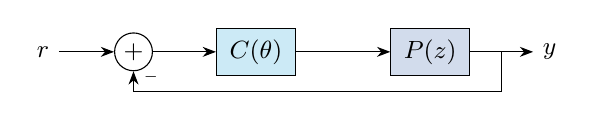
\begin{tikzpicture}[>=Stealth, node distance=1cm, every node/.style={font=\small}]
        \node[draw, rectangle, minimum width=1cm, minimum height=0.6cm, fill=midblue!20] (P) {$P(z)$};
        \node[draw, rectangle, minimum width=1cm, minimum height=0.6cm, fill=accentblue!20, left=1.2cm of P] (C) {$C(\theta)$};
        \node[circle, draw, inner sep=1.5pt, left=0.8cm of C] (sum) {$+$};
        \node[left=0.7cm of sum, font=\small] (r) {$r$};
        \node[right=0.8cm of P, font=\small] (y) {$y$};
        \draw[->] (r) -- (sum);
        \draw[->] (sum) -- (C);
        \draw[->] (C) -- (P);
        \draw[->] (P) -- (y);
        \draw[->] ($(P.east)+(0.4,0)$) -- ++(0,-0.5) -| ($(sum.south)$) node[pos=0.85,right,font=\tiny]{$-$};
      \end{tikzpicture}
    \end{column}
  \end{columns}
\end{frame}

% ══════════════════════════════════════════════════════════════════════════════
\section{The Virtual Reference Idea}
% ══════════════════════════════════════════════════════════════════════════════

\begin{frame}{The Virtual Reference Framework}
  \begin{block}{Core Insight}
    If $C(z;\theta)$ achieves closed-loop TF $= M(z)$, then for any reference $\bar{r}(t)$:
    \[
      y(t) = M(z)\,\bar{r}(t)
    \]
    Turning this around: \emph{given measured $y(t)$, define a ``virtual'' reference}:
    \[
      \bar{r}(t) \text{ such that } M(z)\,\bar{r}(t) = y(t)
    \]
  \end{block}

%  \vspace{0.3em}

  \begin{columns}[T]
    \begin{column}{0.4\textwidth}
      \begin{exampleblock}{Key Observation}
        \begin{itemize}
          \item Tracking error: $e(t) = \bar{r}(t) - y(t)$
          \item $P(z)$ fed by $u(t)$ produces $y(t)$
          \item A \textbf{good} $C$ maps $e(t) \to u(t)$
          \item Both $e(t)$ and $u(t)$ are \highlight{known!}
        \end{itemize}
      \end{exampleblock}
    \end{column}
    \begin{column}{0.4\textwidth}
      \begin{alertblock}{Reduction to Identification}
        Finding $C(z;\theta)$ such that
        \[ C(z;\theta)\,e(t) \approx u(t) \]
        is a \textbf{standard regression problem} --- solvable with no knowledge of $P(z)$.
      \end{alertblock}
    \end{column}
  \end{columns}
\end{frame}

% ─────────────────────────────────────────────────────────────────────────────
\begin{frame}{The VRFT Algorithm (Basic Form)}
  \begin{block}{Three-Step Procedure \quad (noise-free case)}
    Given $\{u(t),\, y(t)\}_{t=1}^{N}$:
    \begin{enumerate}
      \setlength{\itemsep}{0.6em}
      \item \textbf{Compute virtual reference \& tracking error:}
        \[ \bar{r}(t): \quad y(t)=M(z)\bar{r}(t), \qquad e(t)=\bar{r}(t)-y(t) \]
      \item \textbf{Filter both signals with pre-filter $L(z)$:}
        \[ e_L(t) = L(z)\,e(t), \qquad u_L(t) = L(z)\,u(t) \]
      \item \textbf{Solve a least-squares problem:}
        \[ \hat{\theta}_N = \arg\min_\theta \; \frac{1}{N}\sum_{t=1}^{N}\bigl(u_L(t) - C(z;\theta)\,e_L(t)\bigr)^2 \]
        Closed form: $\;\hat{\theta}_N = \left(\sum \varphi_L\varphi_L^T\right)^{-1}\sum \varphi_L\, u_L(t)$
        \quad where $\varphi_L(t)=\beta(z)\,e_L(t)$.
    \end{enumerate}
  \end{block}
\end{frame}

% ══════════════════════════════════════════════════════════════════════════════
\section{Pre-Filter Design}
% ══════════════════════════════════════════════════════════════════════════════

\begin{frame}{Why the Pre-Filter $L(z)$ Matters}
  \begin{columns}[T]
    \begin{column}{0.5\textwidth}
      \begin{block}{Two Cost Functions}
        \textbf{Model-reference criterion:}
        \[
          J_{\mathrm{MR}}(\theta)=\frac{1}{2\pi}\!\int_{-\pi}^{\pi}
          \!\!\left|\frac{PC(\theta)}{1+PC(\theta)}-M\right|^2\!|W|^2 d\omega
        \]
        \vspace{0.2em}
        \textbf{Virtual reference criterion (asymptotic):}
        \[
          J_{\mathrm{VR}}(\theta)=\frac{1}{2\pi}\!\int_{-\pi}^{\pi}
          \!\!\frac{|P|^2|C(\theta)-C_0|^2|1-M|^2|L|^2}{|M|^2}\Phi_u\; d\omega
        \]
      \end{block}
    \end{column}
    \begin{column}{0.47\textwidth}
      \begin{exampleblock}{Ideal (infeasible) choice}
        $J_{\mathrm{VR}} = J_{\mathrm{MR}}$ if:
        \[ |L|^2 = \frac{|M|^2|W|^2}{|1+PC(\theta)|^2}\frac{1}{\Phi_u} \]
        \textit{Not computable — depends on unknown $P$ and on $\theta$.}
      \end{exampleblock}
      \vspace{0.4em}
      \begin{alertblock}{Proposed feasible choice}
        Replace $|1+PC(\theta)|^2$ by $|1+PC_0|^2$:
        \[
          \boxed{|L|^2 = \frac{|1-M|^2\,|W|^2}{|M|^2}\frac{1}{\Phi_u}}
        \]
        \textit{All quantities are \textbf{known}.}
      \end{alertblock}
    \end{column}
  \end{columns}
\end{frame}

% ─────────────────────────────────────────────────────────────────────────────
\begin{frame}{Optimality of the Proposed Filter (Proposition 1)}
  \begin{block}{Setup: Extended Controller Class}
    Let $C_0(z)$ be the \emph{ideal} controller achieving $\frac{PC_0}{1+PC_0}=M(z)$.
    Define $\tilde{C}(z) = C_0(z) - \beta^T(z)\bar{\theta}$\; (unexplained part).\\[0.4em]
    \textbf{Extended class:} $C^+(z;\theta^+) = \beta^+(z)^T\theta^+$, where $\beta^+ = [\beta_1,\ldots,\beta_n,\tilde{C}]^T$.
  \end{block}
  \vspace{0.5em}
  \begin{columns}[T]
    \begin{column}{0.5\textwidth}
      \begin{exampleblock}{Proposition 1}
        With $L(z)$ chosen as above:
        \begin{align*}
          \bar{\theta} &= \arg\min_\theta\; J^+_{\mathrm{MR}}\bigl([\theta^T,0]^T\bigr)\\[0.3em]
          \hat{\theta} &= \arg\min_\theta\; \hat{J}^+_{\mathrm{MR}}\bigl([\theta^T,0]^T\bigr)
        \end{align*}
        where $\hat{J}^+_{\mathrm{MR}}$ is the \emph{quadratic approximation} of $J^+_{\mathrm{MR}}$ around $\bar{\theta}^+$.
      \end{exampleblock}
    \end{column}
    \begin{column}{0.47\textwidth}
      \begin{block}{Interpretation}
        \begin{itemize}
          \item If $C_0 \in \{C(z;\theta)\}$: VRFT finds the \highlight{global optimum} of $J_{\mathrm{MR}}$ exactly
          \item If not (restricted complexity): VRFT finds a \highlight{near-optimal} solution
          \item Near-optimality improves as the controller class better approximates $C_0$
        \end{itemize}
      \end{block}
    \end{column}
  \end{columns}
\end{frame}

% ══════════════════════════════════════════════════════════════════════════════
\section{Handling Noisy Data}
% ══════════════════════════════════════════════════════════════════════════════

\begin{frame}{Effect of Noise on VRFT}
  \begin{block}{Noise Model}
    Measured output: $\tilde{y}(t) = P(z)u(t) + d(t)$, where $u(\cdot)$ and $d(\cdot)$ are \textbf{uncorrelated} (open-loop data).
  \end{block}
  \vspace{0.3em}
  \begin{columns}[T]
    \begin{column}{0.5\textwidth}
      \begin{block}{Asymptotic criterion — noisy case}
        \small
        \[
          J_{\mathrm{VR}}(\theta) = \frac{1}{2\pi}\!\int \!\left[\frac{|P|^2|C(\theta)-C_0|^2|1-M|^2|L|^2}{|M|^2}\Phi_u + \frac{|C(\theta)|^2|P|^2|C_0|^2|L|^2}{\cdot}\Phi_d\right]d\omega
        \]
        The extra noise term \alerttext{biases} the estimator!
      \end{block}
    \end{column}
    \begin{column}{0.47\textwidth}
      \begin{alertblock}{Solution: Instrumental Variables}
        Replace the standard LS estimate with:
        \[
          \hat{\theta}^{\mathrm{IV}}_N = \left(\sum \xi(t)\,\tilde{\varphi}_L^T\right)^{-1}\sum \xi(t)\,u_L(t)
        \]
        where $\xi(t)$ is a suitable \textbf{instrumental variable} uncorrelated with $d(t)$ but correlated with $\varphi_L(t)$.
      \end{alertblock}
    \end{column}
  \end{columns}
\end{frame}

% ─────────────────────────────────────────────────────────────────────────────
\begin{frame}{Instrumental Variable Choices}
  \begin{columns}[T]
    \begin{column}{0.48\textwidth}
      \begin{exampleblock}{Choice 1: Repeated Experiment}
        \begin{itemize}
          \item Run plant again with \emph{same} input $\{u(t)\}$
          \item Collect second output $\{\tilde{y}'(t)\}$
          \item Use: $\xi(t) = \beta(z)L(z)(M^{-1}-1)\tilde{y}'(t)$
        \end{itemize}
        \vspace{0.3em}
        \textbf{Guarantee:} $\hat{\theta}^{\mathrm{IV}} \to \hat{\theta}$ asymptotically\\[0.2em]
        \textbf{Cost:} Requires a second experiment
      \end{exampleblock}
    \end{column}
    \begin{column}{0.48\textwidth}
      \begin{exampleblock}{Choice 2: Plant Model (Preferred)}
        \begin{itemize}
          \item Identify high-order model $\hat{P}(z)$ from data (e.g.\ ARX)
          \item Simulate: $\hat{y}(t) = \hat{P}(z)u(t)$
          \item Use: $\xi(t) = \beta(z)L(z)(M^{-1}-1)\hat{y}(t)$
        \end{itemize}
        \vspace{0.3em}
        \textbf{Guarantee:} Approximately unbiased\\[0.2em]
        \textbf{Note:} Model used \emph{only} for IV generation; its quality does not affect controller complexity
      \end{exampleblock}
    \end{column}
  \end{columns}
  \vspace{0.4em}
  \begin{block}{Remark}
    Even when using Choice 2, VRFT remains \emph{essentially direct}: the identified model $\hat{P}(z)$ is a \textbf{nuisance parameter}, not the design basis.
  \end{block}
\end{frame}

% ─────────────────────────────────────────────────────────────────────────────
\begin{frame}{Complete VRFT Algorithm (with IV)}
  \begin{block}{Summary --- using plant identification for IV}
    \begin{enumerate}
      \setlength{\itemsep}{0.45em}
      \item Set $L(z) = (1-M(z))\,M(z)\,W(z)\,U(z)^{-1}$, where $|U(e^{j\omega})|^2 = \Phi_u(\omega)$
      \item Compute filtered input: $u_L(t) = L(z)\,u(t)$
      \item Compute noisy regressors: $\tilde{\varphi}_L(t) = \beta(z)L(z)(M^{-1}(z)-1)\,\tilde{y}(t)$
      \item Identify high-order model $\hat{P}(z)$ from $\{u(t),\tilde{y}(t)\}$ (e.g.\ ARX)
      \item Compute instrumental variables: $\xi(t) = \beta(z)L(z)(M^{-1}(z)-1)\,\hat{P}(z)u(t)$
      \item Solve:
        \[
          \hat{\theta}^{\mathrm{IV}}_N = \left(\sum_{t=1}^{N}\xi(t)\,\tilde{\varphi}_L(t)^T\right)^{-1}\!\sum_{t=1}^{N}\xi(t)\,u_L(t)
        \]
    \end{enumerate}
  \end{block}
\end{frame}

% ══════════════════════════════════════════════════════════════════════════════
\section{Simulation Example}
% ══════════════════════════════════════════════════════════════════════════════

\begin{frame}{Flexible Transmission Benchmark}
  \begin{columns}[T]
    \begin{column}{0.52\textwidth}
      \textbf{Plant:} Three pulleys connected by elastic belts
      \[
        P(z) = \frac{z^{-3}B(z)}{A(z)}, \quad T_s = 0.05\,\text{s}
      \]
      \textbf{Objective:} Track angular position of 3rd pulley.\\[0.5em]
      \textbf{Reference model:}
      \[
        M(z) = \frac{z^{-3}(1-\alpha)^2}{(1-\alpha z^{-1})^2}, \quad \alpha = e^{-T_s \omega_0}
      \]
      \textbf{Controller class (6 parameters):}
      \[
        C(z;\theta) = \frac{\theta_0 + \theta_1 z^{-1}+\cdots+\theta_5 z^{-5}}{1-z^{-1}}
      \]
      \textbf{Data:} $N=512$ samples, white noise input ($\Phi_u=0.01$)
    \end{column}
    \begin{column}{0.45\textwidth}
      \begin{block}{Three Cases Studied}
        \begin{enumerate}
          \item $L(z)=1$ (trivial filter, no noise)
          \item $L(z) = (1-M)M$ (optimal filter, no noise)
          \item $L(z) = (1-M)M$ (optimal filter, SNR = 10, with IV)
        \end{enumerate}
      \end{block}
      \vspace{0.4em}
      \begin{alertblock}{Key Challenge}
        Plant is \textbf{non-minimum phase} --- perfect model matching would destabilize the loop. Controller must avoid cancelling the unstable zero.
      \end{alertblock}
    \end{column}
  \end{columns}
\end{frame}

% ─────────────────────────────────────────────────────────────────────────────
\begin{frame}{Simulation Results}
  \begin{columns}[T]
    \begin{column}{0.32\textwidth}
      \begin{block}{Case 1: $L(z)=1$}
        \centering
        \vspace{0.2em}
        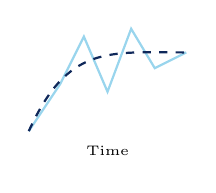
\begin{tikzpicture}
          \draw[accentblue!40, thick] (0,0) -- (0.4,0.6) -- (0.7,1.2) -- (1.0,0.5) -- (1.3,1.3) -- (1.6,0.8) -- (2.0,1.0);
          \draw[darkblue, thick, dashed] (0,0) .. controls (0.5,1.1) and (1.0,1.0) .. (2.0,1.0);
          \node[font=\tiny] at (1.0,-0.25) {Time};
        \end{tikzpicture}\\
        $J_{\mathrm{MR}} = 0.232$\\[0.2em]
        \alerttext{Poor tracking} — control system differs markedly from $M(z)$
      \end{block}
    \end{column}
    \begin{column}{0.32\textwidth}
      \begin{block}{Case 2: Optimal $L(z)$}
        \centering
        \vspace{0.2em}
        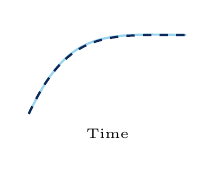
\begin{tikzpicture}
          \draw[accentblue!40, thick] (0,0) .. controls (0.5,1.05) and (0.9,1.02) .. (2.0,1.0);
          \draw[darkblue, thick, dashed] (0,0) .. controls (0.5,1.08) and (1.0,1.0) .. (2.0,1.0);
          \node[font=\tiny] at (1.0,-0.25) {Time};
        \end{tikzpicture}\\
        $J_{\mathrm{MR}} = 0.0343$\\[0.2em]
        \highlight{Near-perfect tracking}\\[0.2em]
        Optimal: $J_{\mathrm{MR}}(\bar\theta)=0.0340$
        \quad\emph{Sub-optimality $<1\%$}
      \end{block}
    \end{column}
    \begin{column}{0.32\textwidth}
      \begin{block}{Case 3: Noisy + IV}
        \centering
        \vspace{0.2em}
        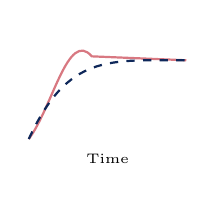
\begin{tikzpicture}
          \draw[alertred!60, thick] (0,0) .. controls (0.3,0.4) and (0.5,1.4) .. (0.8,1.05) -- (2.0,1.0);
          \draw[darkblue, thick, dashed] (0,0) .. controls (0.5,1.08) and (1.0,1.0) .. (2.0,1.0);
          \node[font=\tiny] at (1.0,-0.25) {Time};
        \end{tikzpicture}\\
        Without IV: degraded\\[0.2em]
        \highlight{With IV (ARX model):} performance nearly restored to Case 2
      \end{block}
    \end{column}
  \end{columns}
  \vspace{0.4em}
  \centering
  \small\textit{(Schematic step-response illustrations; solid = achieved, dashed = reference model $M(z)$)}
\end{frame}

% ══════════════════════════════════════════════════════════════════════════════
\section{Comparison \& Conclusions}
% ══════════════════════════════════════════════════════════════════════════════

\begin{frame}{Comparison with Related Methods}
  \begin{center}
  \begin{tabular}{lcccc}
    \toprule
    \textbf{Method} & \textbf{Direct} & \textbf{Iterative} & \textbf{Global Opt.} & \textbf{Single Exp.}\\
    \midrule
    Ziegler--Nichols (1942) & \checkmark & --- & --- & \checkmark \\
    IFT (Hjalmarsson 1994) & \checkmark & \checkmark & local & multiple \\
    CLOE / VRFD          & $\times$ & \checkmark & local & multiple \\
    \textbf{VRFT (this work)} & \checkmark & --- & \highlight{\checkmark} & \checkmark \\
    \bottomrule
  \end{tabular}
  \end{center}
  \vspace{0.5em}
  \begin{columns}[T]
    \begin{column}{0.48\textwidth}
      \begin{block}{VRFT vs.\ IFT}
        \begin{itemize}
          \item Both are \emph{direct} (no model used for design)
          \item IFT: iterative, fine-tuning, locally optimal
          \item VRFT: one-shot, globally (near-)optimal
          \item \highlight{Complementary methods} --- VRFT can initialize IFT
        \end{itemize}
      \end{block}
    \end{column}
    \begin{column}{0.48\textwidth}
      \begin{block}{Advantage over Tuning Rules}
        \begin{itemize}
          \item Not limited to PID
          \item Specifications given via $M(z)$ (flexible)
          \item No pre-specified empirical rule
          \item No parameter initialization needed
        \end{itemize}
      \end{block}
    \end{column}
  \end{columns}
\end{frame}

% ─────────────────────────────────────────────────────────────────────────────
\begin{frame}{Summary \& Key Takeaways}
  \begin{columns}[T]
    \begin{column}{0.55\textwidth}
      \begin{exampleblock}{What VRFT Offers}
        \begin{itemize}
          \setlength{\itemsep}{0.4em}
          \item \textbf{Direct} global minimisation of model-reference criterion from I/O data
          \item \textbf{No plant model} needed for controller design
          \item \textbf{Single experiment}, no iterations, no initialisation
          \item Handles \textbf{restricted-complexity} controller classes with near-optimal guarantees (Prop.~1)
          \item Handles \textbf{noisy data} via instrumental variables
          \item Applicable to any linear controller structure (not just PID)
        \end{itemize}
      \end{exampleblock}
    \end{column}
    \begin{column}{0.42\textwidth}
      \begin{alertblock}{Limitations \& Open Issues}
        \begin{itemize}
          \item Stability of the designed closed-loop is \emph{not} guaranteed --- must be verified separately
          \item Near-optimality depends on how well the controller class approximates $C_0(z)$
          \item IV approach requires an additional data pass or a second experiment
          \item Closed-loop data collection: straightforward extension but not detailed here
        \end{itemize}
      \end{alertblock}
    \end{column}
  \end{columns}
\end{frame}

% ─────────────────────────────────────────────────────────────────────────────
\begin{frame}[plain]
  \begin{center}
    \vspace{1.5em}
    {\Large\color{darkblue}\textbf{Thank You}}\\[1em]
    \rule{0.5\textwidth}{0.5pt}\\[1em]
    \textbf{Reference:}\\[0.4em]
    M.C.~Campi, A.~Lecchini, S.M.~Savaresi\\
    \textit{Virtual Reference Feedback Tuning: a direct method for the design of feedback controllers}\\
    \textbf{Automatica}, 38(8):1337--1346, 2002\\[1.5em]
    \rule{0.5\textwidth}{0.5pt}\\[0.8em]
    {\small Questions?}
  \end{center}
\end{frame}

\end{document}
